\appchapter[RL Agent Training]{RL Agent Training}
\label{appendix:d}

% Phase 1
% We observe that the RL agent converges to 10 interactive threads and 10 batch threads. The results are showing in figure X.

% Phase 2
% We observe that the RL agent converges to 10 interactive threads and 10 batch threads. The results are showing in figure X.

% Phase 3
% We observe that the RL agent converges to 10 interactive threads and 10 batch threads. The results are showing in figure X.

% Phase 4
% We observe that the RL agent converges to 10 interactive threads and 10 batch threads. The results are showing in figure X.

\begin{table}[ht]
    \centering
    \label{table:hyperparameter_tuning}
    % \caption[RL Regression Models: Hyperparameter Tuning]{List of parameters used for tuning hyperparameters of the polynomial regression models used for function approximation. $Degree$ represents the degree of the polynomial function. $Loss$ represents the loss funciton used by stochastic gradient descent. regularizer represents the penalty to applied to the loss function to shrink the model parameters towards the zero vector. This technique is widely used in regression models to avoid overfitting the data. $Alpha$ represent the strenght to whic the regularization penalty is applied. $learning\_rate$ represents the learning rate schedul of the model. $Max_iter$ represents the maximum number of passes over the training dat}
    \caption[Hyperparameter Tuning Options for Polynomial Regression Models]{Overview of hyperparameters used in the tuning process for polynomial regression models employed in function approximation. The $degree$ parameter denotes the degree of the polynomial function utilized. The $loss$ parameter specifies the loss function employed during stochastic gradient descent. The $penalty$ parameter represents the regularization technique applied to mitigate overfitting. The $alpha$ parameter indicates the strength of the regularization penalty. The $learning\_rate$ parameter determines the scheduling of the model's learning rate. Finally, the $max\_iterations$ parameter sets the maximum number of passes over the training data.}
    % Tabular environment goes AFTER the caption!
    % \begin{adjustbox}{width=1\textwidth}
    \begin{tabular}{|c|c|}
      % after \\: \hline or \cline{col1-col2} \cline{col3-col4} ...
      \hline
      \thead{Parameter} & \thead{Values} \\
      \hline
      degree & 1,2,3 \\\hline
      loss & squared, huber, epsilon\_insensitive \\\hline
      penalty & l1, l2, elasticnet \\\hline
      alpha & 0.1, 0.01, 0.001, 0.0001 \\\hline
      learning rate & constant, optimal, invscaling \\\hline
      max\_iterations & 100, 1000, 10000, 100000 \\
      \hline
    \end{tabular}
    % \caption{Model Selection and Hyper-parameter Tuning parameters categorized by type.}
  % \end{adjustbox}
  \end{table}
  
  \begin{table}[ht]
    \centering
    \label{table:per_model_parameters}
    \caption[Resulting Hyperparameters for Polynomial Regression Models]{Hyperparameters of the polynomial regression models after hyperparameter tuning.}
    % Tabular environment goes AFTER the caption!
    \begin{adjustbox}{width=1\textwidth}
    \begin{tabular}{|l|l|}
      % after \\: \hline or \cline{col1-col2} \cline{col3-col4} ...
      \hline
      \thead{Model} & \thead{Parameters} \\
      \hline
      Model\_1 & \makecell[cl] {degree: 2, learning\_rate: 'invscaling', loss: 'squared\_loss', alpha: 0.1, max\_iter: 1000, \\ penalty: elasticnet} \\\hline
        Model\_2 & \makecell[cl] {degree: 2, learning\_rate: 'invscaling', loss: 'squared\_loss', alpha: 0.01, max\_iter: 10000, \\ penalty: l1} \\\hline
        Model\_3 & \makecell[cl] {degree: 2, learning\_rate: 'invscaling', loss: 'squared\_loss', alpha: 0.0001, max\_iter: 100, \\ penalty: elasticnet} \\\hline
        Model\_4 & \makecell[cl] {degree: 2, learning\_rate: 'invscaling', loss: 'squared\_loss', alpha: 0.001, max\_iter: 10000, \\ penalty: l1} \\\hline
          Model\_5 & \makecell[cl] {degree: 2, learning\_rate: 'invscaling', loss: 'squared\_loss', alpha: 0.01, max\_iter: 10000, \\ penalty: elasticnet} \\\hline
      Model\_6 & \makecell[cl] {degree: 2, learning\_rate: 'invscaling', loss: 'squared\_loss', alpha:  0.01, max\_iter: 1000, \\ penalty: elasticnet} \\\hline
      Model\_7 & \makecell[cl] {degree: 2, learning\_rate: 'invscaling', loss: 'squared\_loss', alpha: 0.01, max\_iter: 1000, \\ penalty: elasticnet} \\\hline
      Model\_8 & \makecell[cl] {degree: 2, learning\_rate: 'invscaling', loss: 'squared\_loss', alpha: 0.1, max\_iter: 10000, \\ penalty: l1} \\\hline
      Model\_9 & \makecell[cl] { degree: 2, learning\_rate: 'invscaling', loss: 'squared\_loss', alpha: 0.01, max\_iter: 100, \\ penalty: elasticnet} \\
      \hline
    \end{tabular}
  \end{adjustbox}
  \end{table}
  
  \begin{table}[ht]
    \centering
    \label{table:rl_training_parameters}
    \caption[Q-Learning Parameters]{Parameters utilized for Q-Learning by the RL agent. The target 99th percentile latency and throughput represent predefined SLAs guiding the reward calculation. The aim is to maintain the observed 99th percentile latency below 250 microseconds while ensuring throughput remains above 250,000 operations per second. The exploration rate ($epsilon$) diminishes gradually between episodes, following a decay rate ($epsilon\_decay$), to strike a balance between exploration and exploitation of knowledge. Furthermores, additional episodes beyond the initially specified count are introduced to enable the agent to reach the optimal policy for phases 1, 3, and 4.}
    % Tabular environment goes AFTER the caption!
    % \begin{adjustbox}{width=1\textwidth}
    \begin{tabular}{|c|c|}
      % after \\: \hline or \cline{col1-col2} \cline{col3-col4} ...
      \hline
      \thead{Parameter} & \thead{Value} \\
      \hline
      episodes & Phases $1,3,4$: 1,000, Phase $2$: 700 \\\hline
      steps per episode & 200 \\\hline
      gamma & 0.95 \\\hline
      learning rate & 0.7 \\\hline
      epsilon & 0.9 \\\hline
      epsilon\_decay & 0.1 \\\hline
      Target 99th Latency & $\leq$ 250 microseconds \\\hline
      Target throughput & $\geq$ 250,000 operations/second \\
      \hline
    \end{tabular}
  % \end{adjustbox}
  \end{table}

  \begin{table}[ht]
    \centering
    % \caption{Preliminary Rewards Phase 1}
    \caption[Preliminary Measurements for Phase 1]{Experimental reward analysis conducted on Phase 1 using the NVM Middleware with various fixed combinations of threads. The table displays statistics on rewards obtained under different configurations, denoted as I5/B5, I10/B10, I15/B15, I15/B5, and I5/B15. The values represent the distribution of rewards, ranging from the minimum to the maximum observed, along with quartiles and median scores. Based on these preliminary findings, the configuration with 10 interactive threads and 10 batch threads appears to yield the most favorable results for Phase 1.}
    \label{table:rewards_phase_1}
    % Tabular environment goes AFTER the caption!
    % \begin{adjustbox}{width=1\textwidth}
    \begin{tabular}{|c|c|c|c|c|c|}
      % after \\: \hline or \cline{col1-col2} \cline{col3-col4} ...
      \hline
      \thead{} & \thead{I5/B5} & \thead{I10/B10} & \thead{I15/B15} & \thead{I15/B5} & \thead{I5/B15}\\
      \hline
      Min & -5716 & -8312 & -41660 & -5682 & -9436\\\hline
      Q1 & -1383 & 2.7 & -4797 & -2971 & -1\\\hline
      Median & -171 & 3.92 & -2 & -1850 & 0\\\hline
      Q3 & 0 & 4.3 & 3 & -1035 & 1\\\hline
      Max & 1 & 5 & 5 & 3 & 2\\
      \hline
    \end{tabular}
  % \end{adjustbox}
  \end{table}

  \begin{table}[ht]
    \centering
    % \caption{Preliminary Rewards Phase 2}
    \caption[Preliminary Measurements for Phase 2]{Experimental reward analysis conducted on Phase 2 using the NVM Middleware with various fixed combinations of threads. The table displays statistics on rewards obtained under different configurations, denoted as I5/B5, I10/B10, I15/B15, I15/B5, and I5/B15. The values represent the distribution of rewards, ranging from the minimum to the maximum observed, along with quartiles and median scores. Based on these preliminary findings, the configuration with 10 interactive threads and 10 batch threads appears to yield the most favorable results for Phase 2.}
    \label{table:rewards_phase_2}
    % Tabular environment goes AFTER the caption!
    % \begin{adjustbox}{width=1\textwidth}
    \begin{tabular}{|c|c|c|c|c|c|}
      % after \\: \hline or \cline{col1-col2} \cline{col3-col4} ...
      \hline
      \thead{} & \thead{I5/B5} & \thead{I10/B10} & \thead{I15/B15} & \thead{I15/B5} & \thead{I5/B15}\\
      \hline
      Min & -4320 & -7763 & -20455 & -5328 & -10060\\\hline
      Q1 & -463 & -1.9 & -1169 & -368 & 1\\\hline
      Median & 1.3 & 5.2 & 4.2 & 3.1 & 3\\\hline
      Q3 & 1.8 & 5.8 & 4.9 & 3.3 & 4\\\hline
      Max & 2.8 & 6 & 6 & 3.8 & 6\\
      \hline
    \end{tabular}
  % \end{adjustbox}
  \end{table}

  \begin{table}[ht]
    \centering
    % \caption{Preliminary Rewards Phase 3}
    \caption[Preliminary Measurements for Phase 3]{Experimental reward analysis conducted on Phase 3 using the NVM Middleware with various fixed combinations of threads. The table displays statistics on rewards obtained under different configurations, denoted as I5/B5, I7/B3, I7/B7, I10/B10, I15/B15, I15/B5, and I5/B15. The values represent the distribution of rewards, ranging from the minimum to the maximum observed, along with quartiles and median scores. Based on these preliminary findings, the configuration with 7 interactive threads and 3 batch threads appears to yield the most favorable results for Phase 3.}
    \label{table:rewards_phase_3}
    % Tabular environment goes AFTER the caption!
    % \begin{adjustbox}{width=1\textwidth}
    \begin{tabular}{|c|c|c|c|c|c|c|c|}
      % after \\: \hline or \cline{col1-col2} \cline{col3-col4} ...
      \hline
      \thead{} & \thead{I5/B5} & \thead{I7/B3} & \thead{I7/B7} & \thead{I10/B10} & \thead{I15/B15} & \thead{I15/B5} & \thead{I5/B15}\\
      \hline
      Min & -12490 & -6582 & -174852 & -141354 & -149647 & -96900 & -13211\\\hline
      Q1 & -1230 & -1727 & -2567 & -18768 & -42951 & -58414 & -8583\\\hline
      Median & -272 & -672 & -4 & -566 & -14008 & -2954 & -4940\\\hline
      Q3 & -5 & -3 & -2 & -1 & -4607 & 0 & -2709\\\hline
      Max & -3 & -1 & 0 & 3 & -1 & 4 & -943\\
      \hline
    \end{tabular}
  % \end{adjustbox}
  \end{table}

  \begin{table}[ht]
    \centering
    % \caption{Preliminary Rewards Phase 4}
    \caption[Preliminary Measurements for Phase 4]{Experimental reward analysis conducted on Phase 4 using the NVM Middleware with various fixed combinations of threads. The table displays statistics on rewards obtained under different configurations, denoted as I5/B5, I10/B10, I15/B15, and I15/B5. The values represent the distribution of rewards, ranging from the minimum to the maximum observed, along with quartiles and median scores. Based on these preliminary findings, the configuration with 15 interactive threads and 5 batch threads appears to yield the most favorable results for Phase 4.}
    \label{table:rewards_phase_4}
    % Tabular environment goes AFTER the caption!
    % \begin{adjustbox}{width=1\textwidth}
    \begin{tabular}{|c|c|c|c|c|}
      % after \\: \hline or \cline{col1-col2} \cline{col3-col4} ...
      \hline
      \thead{} & \thead{I5/B5} & \thead{I10/B10} & \thead{I15/B15} & \thead{I15/B5}\\
      \hline
      Min & -11341 & -14699 & -21259 & -3912\\\hline
      Q1 & -153 & -2.5 & -6908 & -1\\\hline
      Median & -2 & 2.3 & -3117 & 3\\\hline
      Q3 & 0 & 3.7 & -4 & 4\\\hline
      Max & 3 & 5 & 3 & 5\\
      \hline
    \end{tabular}
  % \end{adjustbox}
  \end{table}

  \begin{figure}[ht]
    \centering
    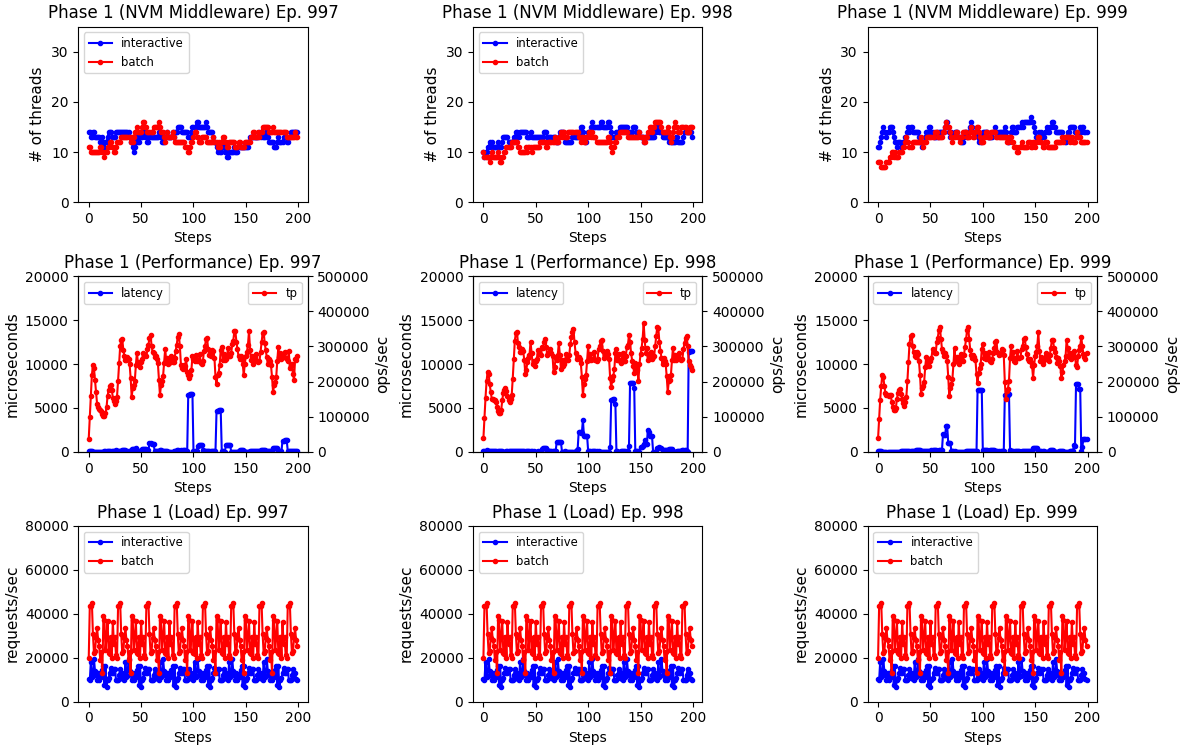
\includegraphics[width=\textwidth,height=\textheight,keepaspectratio,angle=0]{images/rl_training_phase1.png}
    % \caption[Phase 1: Agent's Learned Pattern]{Analysis of the three last episodes of the Q-Learning process performed by the agent when running Phase 1 for 1,000 episodes. On these episodes, the exploration rate is low, indicating that the agent is exploiting its knowledge acquired from previous episodes. The first row demonstrated that the agent configures the NVM Middleware with 10 interactive and 10 batch threads when it starts receiving requests sent from applications configured in Phase 1. This combination of threads matches the preliminary resutls obtained for this phase. Additionally, the second row demonstrates how by configuring the NVM Middleware with the optiomal combination of threads, the agent, most of the steps, keeps the latency low (less than 250 microseconds) and the throughput below 250,000 operations/second.}
    \caption[Learned Pattern of Agent during Phase 1]{Visualization depicting the learned pattern of the agent during Phase 1 of the training process. The analysis focuses on the behavior observed in the final three episodes of the Q-Learning process, which spanned 1,000 episodes. During these episodes, the exploration rate is so low that the agent predominantly exploits its accumulated knowledge. The first row illustrates the agent's configuration of the NVM Middleware with approximately 10 interactive and 10 batch threads, aligning with preliminary results for Phase 1. In the middle row, the throughput and 99th percentile latency reported by the NVM Middleware at each time step are depicted. By employing the optimal combination of threads, the agent consistently maintains low latency (less than 250 microseconds) and a throughput exceeding 250,000 operations/second across most steps. Finally, the bottom row illustrates the operations per second sent to the NVM Middleware by Phase 1.}
    \label{fig:learned_phase_1}
  \end{figure}

  \begin{figure}[ht]
    \centering
    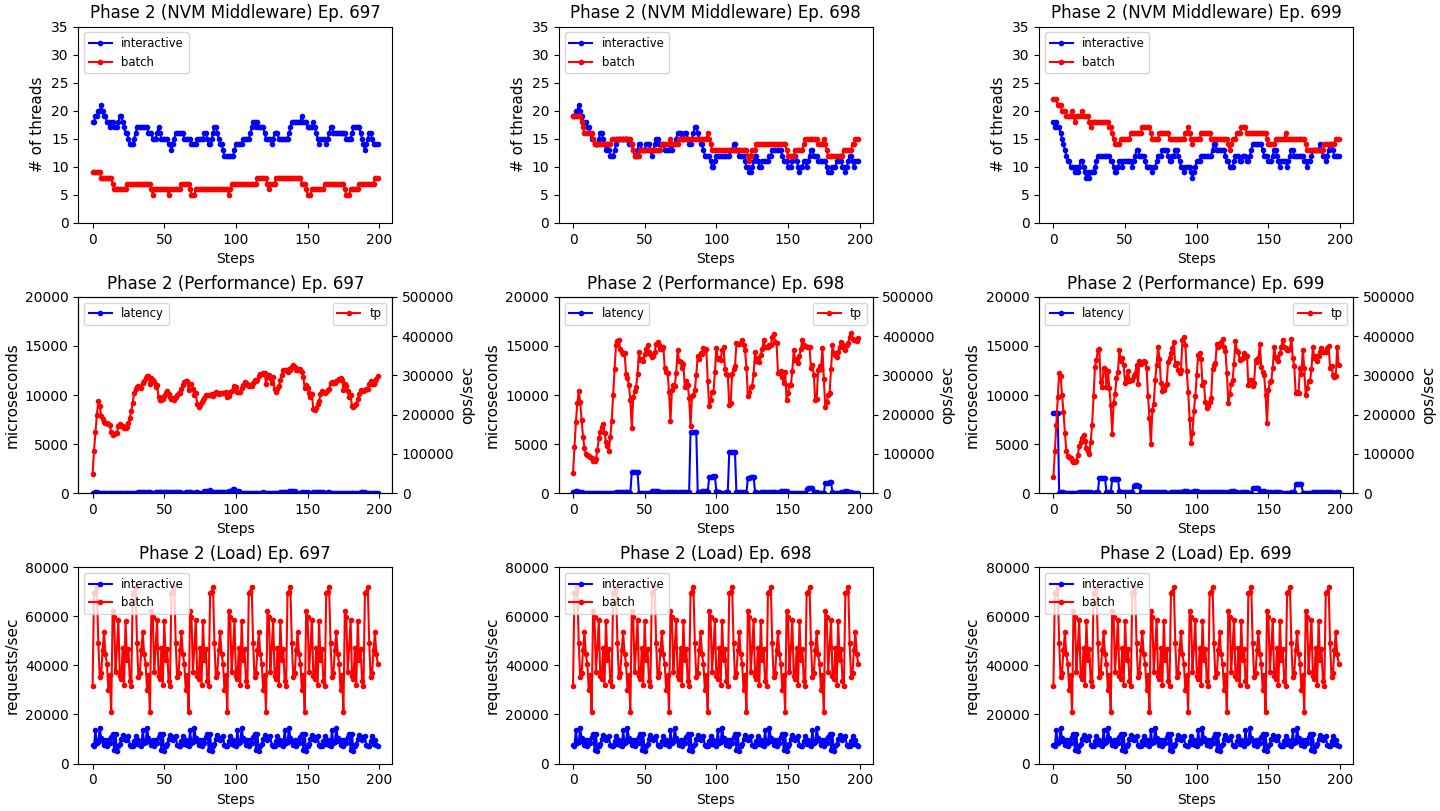
\includegraphics[width=\textwidth,height=\textheight,keepaspectratio,angle=0]{images/rl_training_phase2.png}
    % \caption{Learned Pattern Phase 2}
    \caption[Learned Pattern of Agent during Phase 2]{Visualization depicting the learned pattern of the agent during Phase 2 of the training process. The analysis focuses on the behavior observed in the final three episodes of the Q-Learning process, which spanned 700 episodes. During these episodes, the exploration rate is so low that the agent predominantly exploits its accumulated knowledge. The first row illustrates the agent's configuration of the NVM Middleware with high number of interactive and batch threads (between 10-15), aligning with preliminary results for Phase 2. In the middle row, the throughput and 99th percentile latency reported by the NVM Middleware at each time step are depicted. By employing the optimal combination of threads, the agent consistently maintains low latency (less than 250 microseconds) and a throughput exceeding 250,000 operations/second across most steps. Finally, the bottom row illustrates the operations per second sent to the NVM Middleware by Phase 2.}
    \label{fig:learned_phase_2}
  \end{figure}

  \begin{figure}[ht]
    \centering
    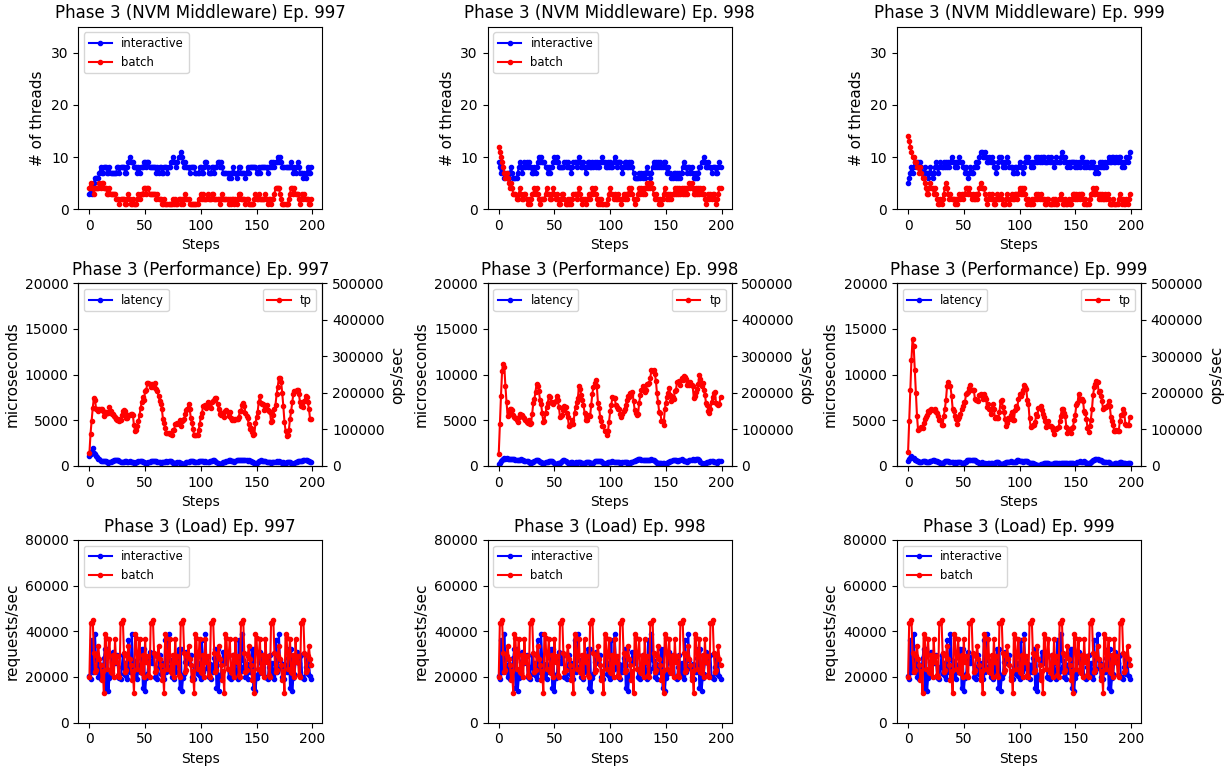
\includegraphics[width=\textwidth,height=\textheight,keepaspectratio,angle=0]{images/rl_training_phase3.png}
    % \caption{Learned Pattern Phase 3}
    \caption[Learned Pattern of Agent during Phase 3]{Visualization depicting the learned pattern of the agent during Phase 1 of the training process. The analysis focuses on the behavior observed in the final three episodes of the Q-Learning process, which spanned 1,000 episodes. During these episodes, the exploration rate is so low that the agent predominantly exploits its accumulated knowledge. The first row illustrates the agent's configuration of the NVM Middleware with approximately 8 interactive and low number of batch threads (approximately less than 5), aligning with preliminary results for Phase 3. In the middle row, the throughput and 99th percentile latency reported by the NVM Middleware at each time step are depicted. By employing the optimal combination of threads, the agent consistently maintains low latency (less than 250 microseconds) and a throughput exceeding 250,000 operations/second across most steps. Finally, the bottom row illustrates the operations per second sent to the NVM Middleware by Phase 3.}
    \label{fig:learned_phase_3}
  \end{figure}

  \begin{figure}[ht]
    \centering
    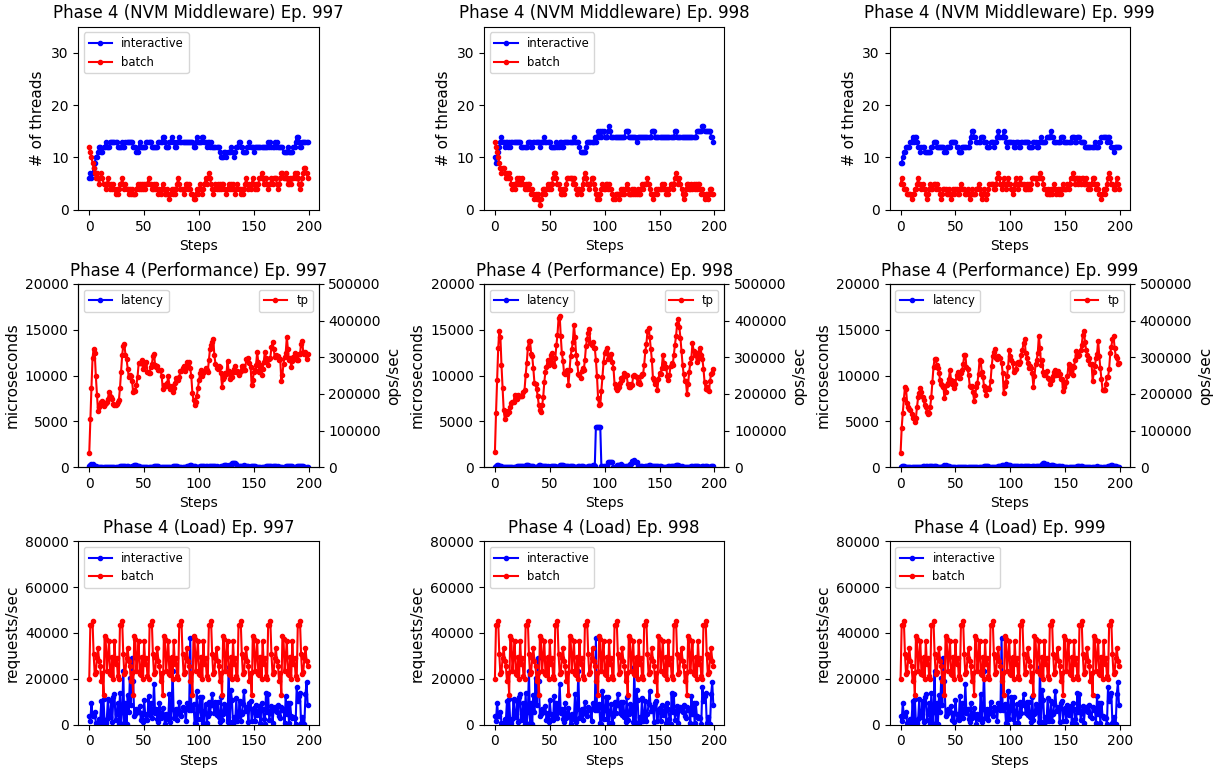
\includegraphics[width=\textwidth,height=\textheight,keepaspectratio,angle=0]{images/rl_training_phase4.png}
    % \caption{Learned Pattern Phase 4}
    \caption[Learned Pattern of Agent during Phase 3]{Visualization depicting the learned pattern of the agent during Phase 1 of the training process. The analysis focuses on the behavior observed in the final three episodes of the Q-Learning process, which spanned 1,000 episodes. During these episodes, the exploration rate is so low that the agent predominantly exploits its accumulated knowledge. The first row illustrates the agent's configuration of the NVM Middleware with high number of interactive threads (approximately 15) and low number of batch threads (approximately 5), aligning with preliminary results for Phase 4. In the middle row, the throughput and 99th percentile latency reported by the NVM Middleware at each time step are depicted. By employing the optimal combination of threads, the agent consistently maintains low latency (less than 250 microseconds) and a throughput exceeding 250,000 operations/second across most steps. Finally, the bottom row illustrates the operations per second sent to the NVM Middleware by Phase 4.}
    \label{fig:learned_phase_4}
  \end{figure}